\chapter{Rupture API via Web UI}\label{rupture_api}

In this chapter we describe our contributions regarding a RESTful API for Rupture.
We believe that the API enables researchers to fully automate 
TLS-based attacks such as compression side-channel attacks. We
provide a usable, clean set of end-points which can be used to mount the
attack. The RESTful API provides managing targets such as various web services,
victims by robustly injecting and sniffing for information on local networks based on IP
addresses and strategies for advancing attack rounds based on state
search exploration. Is also runs analyses on collected data, which is stored
persistently. We are confident this automation will enable cryptographers and
security researchers to heavily experiment with the various attack parameters,
yielding better attack results in terms of correctness and performance.

\section{RESTful API}
In this section, We describe the implementation of a RESTful API via HTTP 
to which the user makes requests from the web User Interface. This 
RESTful API can also be directly used by programmers without the need 
to use the web interface.

\subsection{/attack}

The \textit{/attack} is an HTTP POST endpoint. 

When the backend receives a POST request, it initiates a new attack.
The arguments passed are the victim's IP and the target. There is also an optional
parameter, the \textit{victim\_id}. If the \textit{victim\_id} is set,
the victim already exists. If no \textit{victim\_id} argument is passed, the backend 
creates and stores a new victim. In both cases, the backend
creates the client and injection code for the specific victim and 
injects the client code to the victim's machine with bettercap. 
It returns \textit{HTTP 200} with a JSON that has a 
field \textit{victimid}, which contains the ID of the new victim.

\subsection{/victim}

The \textit{/victim} is an HTTP POST and GET endpoint. 

When the backend receives a POST request, it creates a new victim. 
The argument passed is the victim's IP. The backend 
creates and stores a new victim, and  returns HTTP 200 with a JSON that has a 
field \textit{victimid}, which contains the ID of the new victim.


On a GET request, the backend returns an HTTP 200 JSON response. 
The JSON contains a list of all the stored victims that the attack 
is still running on or has been completed.

\subsection{/victim/$ <victimId> $}

The /victim/$ <victimId> $ is an HTTP GET, PUT and DELETE endpoint.

On a GET request, the backend returns HTTP 200 with a JSON with details 
for the victim with the specific victimId. The argument passed is the 
victim's Id. The backend returns the general information and details of 
the attack. The general information consists of the victim's IP and 
machine name, the target name, the decrypted secret up to this point 
and a percentage of the progress. Percentage is calculated by dividing the
length of the already decrypted-known secret with the length of the whole secret which 
we want to decrypt. Further details are provided per  batch.
These are the round number, the batch number, the alignment alphabet, 
the possible knownsecret and the confidence.

On a PUT request, the user asks the backend to pause or continue the attack. 
The argument passed is the desired state of the attack, either "paused" 
or "running". The backend updates the current state of the attack and 
returns HTTP 200. 

On a DELETE request, the backend deletes the specific attack.

\subsection{/victim/notstarted}

The \textit{/victim/notstarted} is an HTTP GET endpoint. When a GET request 
is received, the backend scans the wifi network with bettercap to find all 
possible victims and their machine's name. The backend returns a list of 
possible's victims IPs and machine names, which are available on the network
but are not already attacked.


\subsection{/target}
This is an HTTP 200 POST and GET endpoint.
On a POST request, the argument passed to the backend is the name of the target, 
the endpoint, the known prefix, the secret's alphabet, the secret length, 
the alignment alphabet, the records' cardinality and the method of the attack. 
The backend creates and stores the new target and returns HTTP 200 with a JSON 
with the target name.

On a GET request, the backend returns an HTTP 200 JSON response. The JSON contains 
a list of all the stored target for which an attack is possible.



\section{Web UI}                                                                                                          

The user handles the attacks via a web interface which consists 
of two main pages and a modal window. The two main pages are the
\textbf{Network Overview} and the \textbf{Victim Attack Inspection}. 
The modal window is used for the target configuration.

The Network Overview is the start page. It displays the completed,
 the currently running and the paused attacks. It also allows the user 
to initiate a new attack either by adding a custom victim or by scanning 
and choosing one of victims with bettercap.

\begin{figure}[H] \caption{Start Page} \centering
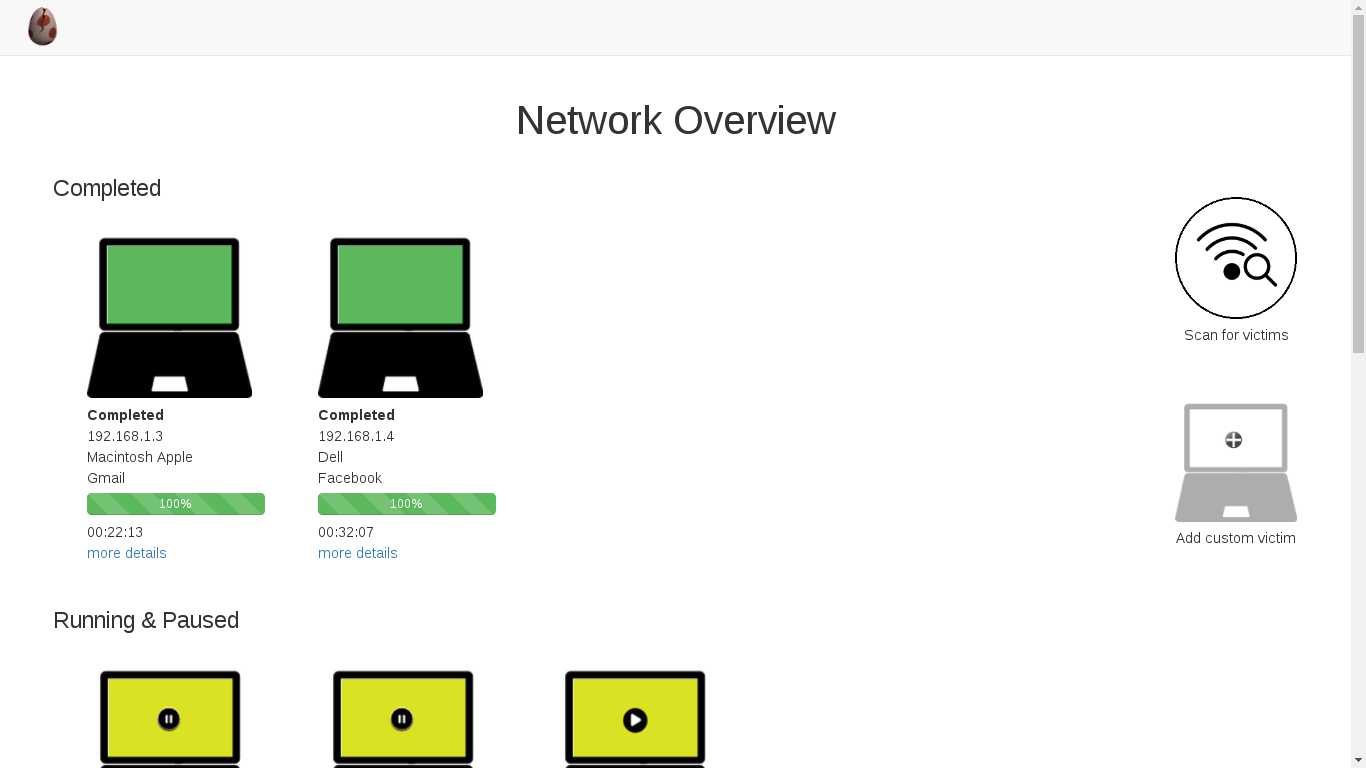
\includegraphics[width=0.7\textwidth]{diagrams/startPage.png}
\end{figure}

The completed and the running or paused attacks are represented by PC icons. 
When the user clicks the \textit{Scan for victims} button, bettercap scans 
the network for possible victims, which are shown beneath the running/paused attacks.
The user can otherwise click on the \textit{Add custom victim} 
button if they already know the victim’s IP and don’t need to search for other victims.

\begin{figure}[H] \centering 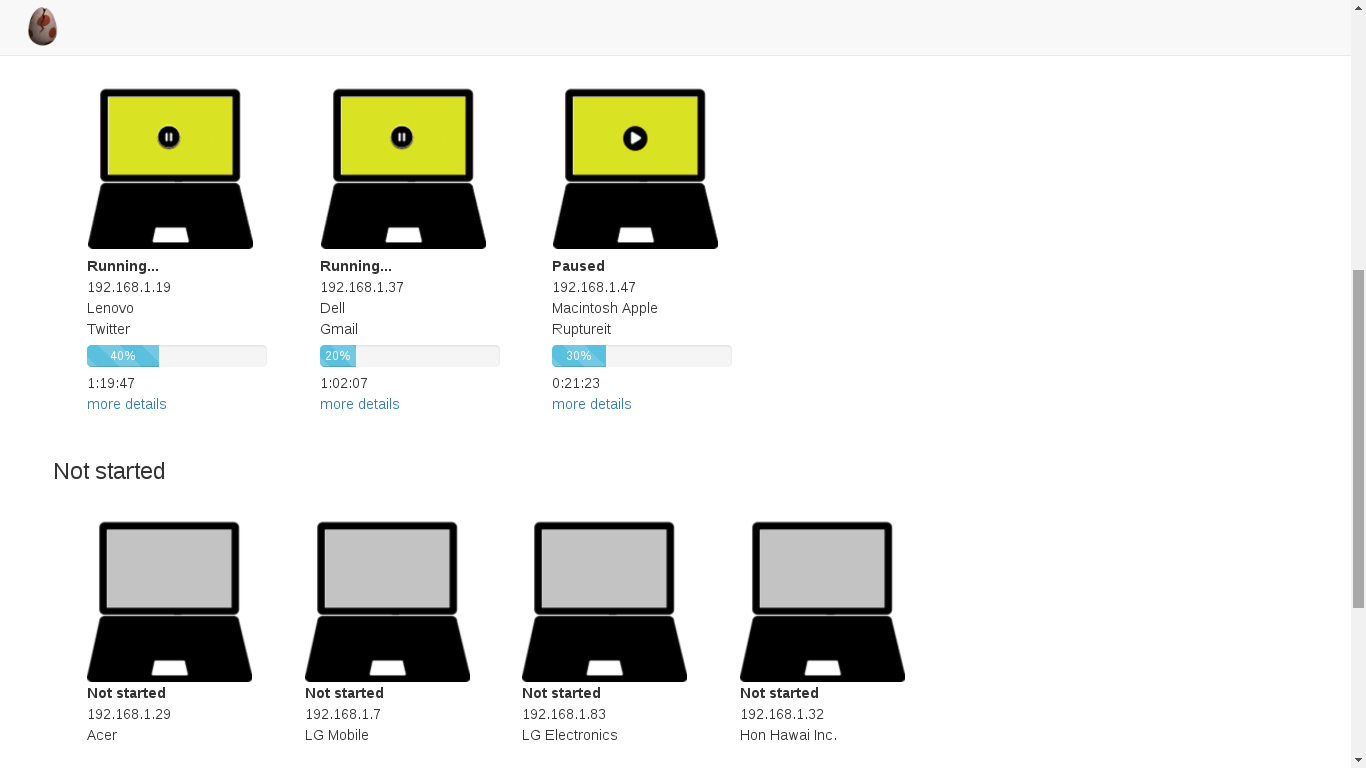
\includegraphics[width=95mm]{diagrams/notstarted.png}
\caption{Possible victims for a new attack} \end{figure}

The victim and target configuration are shown below. If the user has previously scanned 
the network, the victim's IP is already filled.

\begin{figure}[H] \caption{Victim Configuration} \centering 
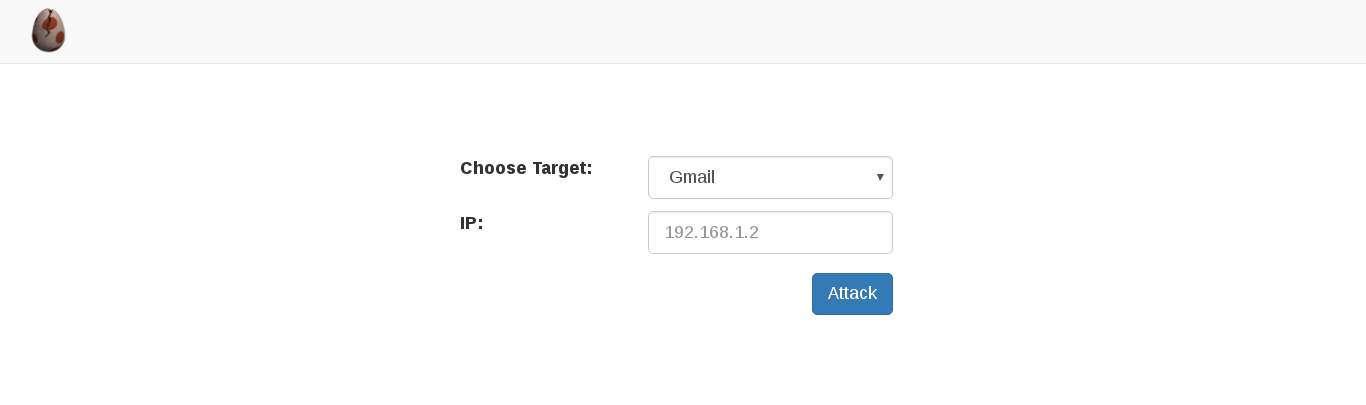
\includegraphics[width=95mm]{diagrams/victim.png} \end{figure}

There are some pre-configured targets but the user can configure a 
new one.


\begin{figure}[H]
    \centering
    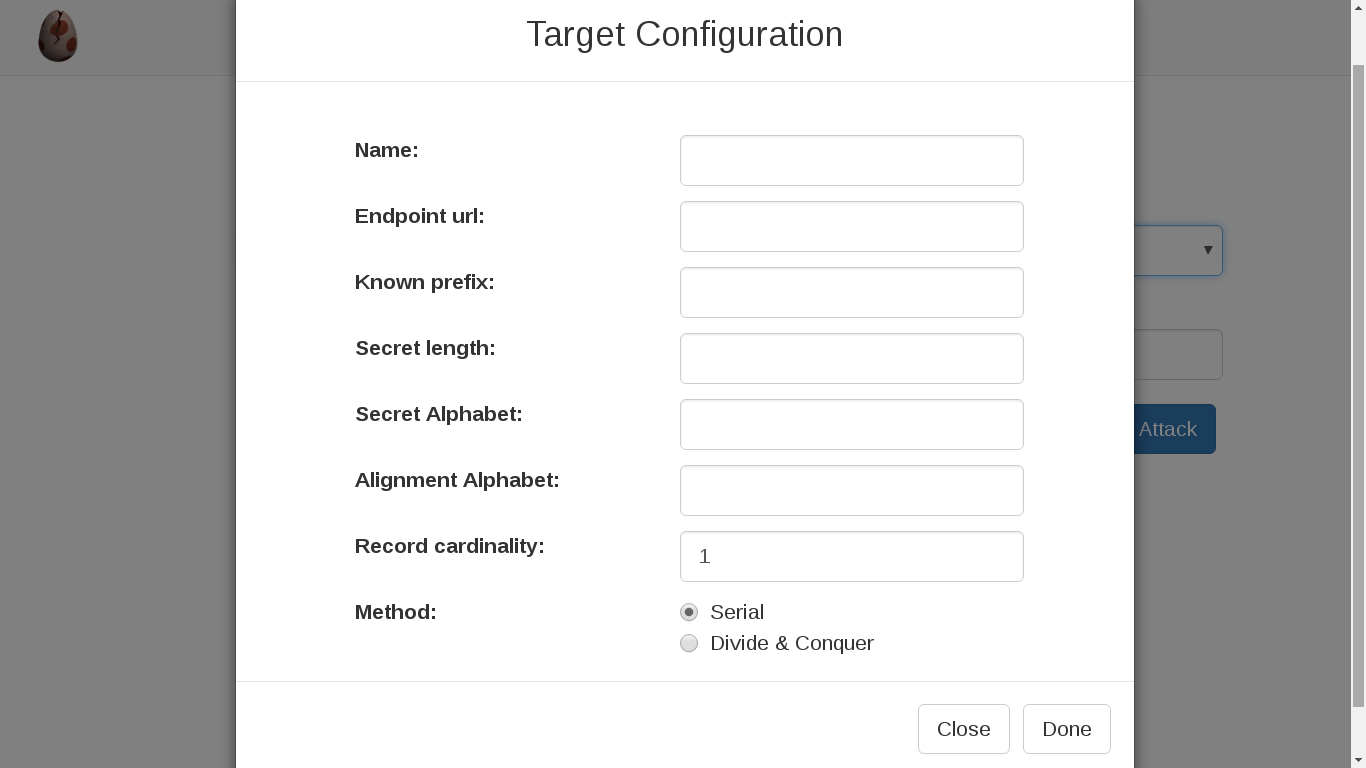
\includegraphics[width=90mm]{diagrams/target.png}
    \caption{Target Configuration}
\end{figure}

When the user clicks on a completed, running or paused attack, 
they can view further details of the attack.

\begin{figure}[H]
    \centering
    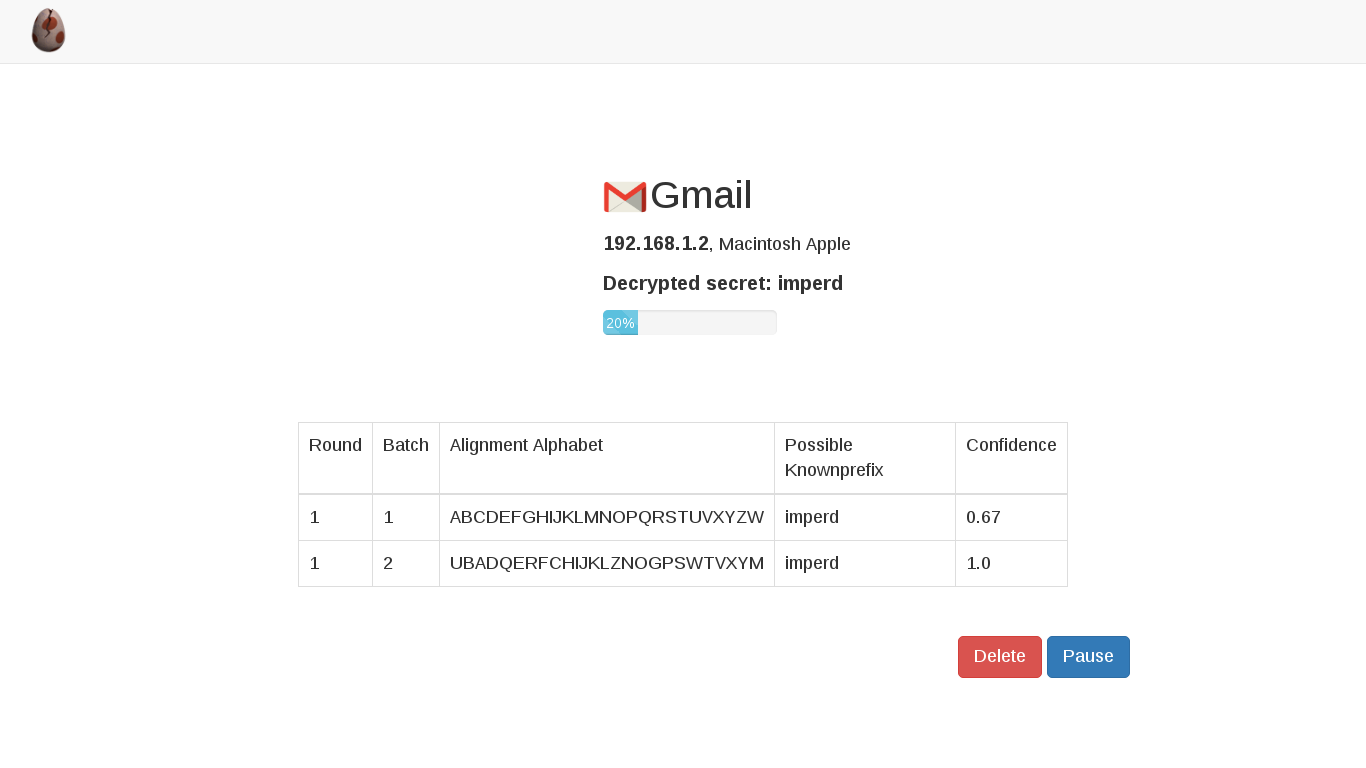
\includegraphics[width=115mm, height=75mm]{diagrams/attack.png}
    \caption{Attack details}
\end{figure}

The above indicate how easily the user can perform the attack in a fully automated way.
